\documentclass[twoside]{article}
\setlength{\oddsidemargin}{0 in}
\setlength{\evensidemargin}{0 in}
\setlength{\topmargin}{-0.6 in}
\setlength{\textwidth}{6.5 in}
\setlength{\textheight}{8.5 in}
\setlength{\headsep}{0.75 in}
\setlength{\parindent}{0 in}
\setlength{\parskip}{0.1 in}

\usepackage{url}
\usepackage{titlesec}
\setcounter{secnumdepth}{3}
\usepackage{palatino}
\usepackage{marginnote}
\usepackage{multirow}
\usepackage{easybmat,bigdelim,arydshln}
\usepackage[authoryear,round]{natbib}
\usepackage{amssymb,amsmath,amsthm,amsfonts}
\usepackage{mathtools}
\usepackage{caption}
\usepackage{hyperref}
\usepackage{tcolorbox}
\tcbuselibrary{skins, breakable, theorems}
\usepackage{newpxtext,newpxmath}
\usepackage{longtable}
\usepackage{enumitem}
\makeatletter

\let\bar\overline

\setlist[itemize]{topsep=0pt,leftmargin=10pt,itemsep=-0.2em}
\usepackage{xcolor}
\usepackage{tikz}
\usepackage{pgfplots}
\pgfplotsset{compat = newest}
\usetikzlibrary{patterns,decorations.pathreplacing,decorations.markings}
\usepgfplotslibrary{fillbetween}

\hypersetup{
    colorlinks,
    citecolor=red,
    filecolor=black,
    linkcolor=violet,
    urlcolor=blue
}

\makeatletter
\renewcommand{\thefigure}{\thesection.\arabic{figure}}
\newtheoremstyle{indented}
  {3pt}% space before
  {3pt}% space after
  {\addtolength{\@totalleftmargin}{3.5em}
   \addtolength{\linewidth}{-3.5em}
   \parshape 1 3.5em \linewidth}% body font
  {}% indent
  {\bfseries}% header font
  {.}% punctuation
  {.5em}% after theorem header
  {}% header specification (empty for default)
\makeatother

\theoremstyle{definition}
\newtheorem{defin}{Definition}[section] % Creates a new counter, number within section
\newtheorem{prt}[defin]{Remark} 
\newtheorem{prts}[defin]{Remarks} % Again share defin's counter
\newtheorem{exmp}[defin]{Example} % etc.
\newtheorem{exmps}[defin]{Examples}
\newtheorem*{note}{Note}
\tcbuselibrary{theorems}

% use counter*=defin to make each tcbtheorem share defin's counter

\newtcbtheorem[use counter*=defin, number within=section]{definition}{Key takeaways}{enhanced, breakable,
    colback = white, colframe = red!55!black, colbacktitle = red!55!black, attach boxed title to top left = {yshift = -2.5mm, xshift = 3mm}, boxed title style = {sharp corners},fonttitle=\bfseries}{takeaway}

\newtcbtheorem[use counter*=defin, number within=section]{theorem}{Theorem}{enhanced, breakable,
    colback = white, colframe = blue!45!black, colbacktitle = blue!45!black, attach boxed title to top left = {yshift = -2.5mm, xshift = 3mm}, boxed title style = {sharp corners},fonttitle=\bfseries}{thm}
    
\newtcbtheorem[use counter*=defin, number within=section]{proposition}{Proposition}{enhanced, breakable,
    colback = white, colframe = teal, colbacktitle = teal, attach boxed title to top left = {yshift = -2.5mm, xshift = 3mm}, boxed title style = {sharp corners},fonttitle=\bfseries}{prop}

\newtcolorbox{example}[1]{enhanced, breakable, colback = white, colframe = orange!85!black, colbacktitle = orange!85!black, attach boxed title to top left = {yshift = -2.5mm, xshift = 3mm}, boxed title style = {sharp corners},fonttitle=\bfseries, title={Example: #1}}

\newtcbox{\myhl}[1][white]
  {on line, arc = 0pt, outer arc = 0pt,
    colback = #1!20!white, colframe = #1!50!black,
    boxsep = 0pt, left = 1pt, right = 1pt, top = 1pt, bottom = 1pt, boxrule = 0pt, bottomrule =0pt, toprule =0pt}
    
\newtcbox{\myhlrule}[1][white]
  {on line, arc = 0pt, outer arc = 0pt,
    colback = #1!20!white, colframe = #1!50!black,
    boxsep = 0pt, left = 1pt, right = 1pt, top = 1pt, bottom = 1pt, boxrule = 0pt, bottomrule =0.5pt, toprule =0.5pt}
%
% The following commands set up the lecnum (lecture number)
% counter and make various numbering schemes work relative
% to the lecture number.
%
\newcounter{lecnum}
\renewcommand{\thepage}{\thelecnum-\arabic{page}}
\renewcommand{\thesection}{\thelecnum.\arabic{section}}
\renewcommand{\theequation}{\thelecnum.\arabic{equation}}
\renewcommand{\thefigure}{\thelecnum.\arabic{figure}}
\renewcommand{\thetable}{\thelecnum.\arabic{table}}

\newcommand{\sidenotes}[1]{\marginnote{\raggedright\scriptsize#1}}
%
% The following macro is used to generate the header.
%
\newcommand{\lecture}[4]{
   \pagestyle{myheadings}
   \thispagestyle{plain}
   \newpage
   \setcounter{lecnum}{#1}
   \setcounter{page}{1}
   \noindent
   \begin{center}
   \framebox{
      \vbox{\vspace{2mm}
    \hbox to 6.28in { {\bf ECON203: Principles of Microeconomics
	\hfill Fall 2022} }
       \vspace{4mm}
       \hbox to 6.28in { {\Large \hfill Note #1: #2  \hfill} }
       \vspace{2mm}
       \hbox to 6.28in { {\it Lecturer: #3 \hfill TA: #4} }
      \vspace{2mm}}
   }
   \end{center}
   \markboth{Week #1: #2}{Week #1: #2}

   {\bf Key points}: {\begin{itemize}
       \item Decision tables give all the information needed to make a decision
       \item Production function tables and labor inputs give all the information needed to figure out trading in this setting.
       \item Be careful with math deductions, but focus more on the intuition :)
   \end{itemize}}

   {\bf Disclaimer}: {\it These notes are written by Sai Zhang for ECON203, based on the problem sets written by Prof. Brijesh Pinto, the instructor of the course. Please do \textbf{NOT} distribute them online without permission.}
   \vspace*{4mm}
}
%

\tikzset{-stealth-/.style={decoration={
  markings,
  mark=at position #1 with {\arrow{stealth}}},postaction={decorate}}}

  \tikzset{tangent/.style={
    decoration={
        markings,% switch on markings
        mark=
            at position #1
            with
            {
                \coordinate (tangent point-\pgfkeysvalueof{/pgf/decoration/mark info/sequence number}) at (0pt,0pt);
                \coordinate (tangent unit vector-\pgfkeysvalueof{/pgf/decoration/mark info/sequence number}) at (1,0pt);
                \coordinate (tangent orthogonal unit vector-\pgfkeysvalueof{/pgf/decoration/mark info/sequence number}) at (0pt,1);
            }
    },
    postaction=decorate
},
use tangent/.style={
    shift=(tangent point-#1),
    x=(tangent unit vector-#1),
    y=(tangent orthogonal unit vector-#1)
},
use tangent/.default=1}

\begin{document}
\lecture{1}{Questions in PS1 and PS2}{Brijesh Pinto}{Sai Zhang}
%\footnotetext{These notes are partially based on those of Nigel Mansell.}

\section{NB (net benefit), OC (opportunity cost), ER (economic rent)}

Consider this general decision table:
\begin{table}[h]
    \centering
    \begin{tabular}{c|c|c}
        Alternative & Willingness to pay (WTP) & Explicit cost (EC) \\
        \hline
        Choice 1 & $WTP_1$ & $EC_1$ \\
        Choice 2 & $WTP_2$ & $EC_2$ \\
        Choice 3 & $WTP_3$ & $EC_3$
    \end{tabular}
    \caption{A general decision table}
    \label{tab:dec_tab}
\end{table}

Then we can have
\begin{itemize}
    \item[-] \myhl[red!55!black]{\textbf{Net benefit}} ($NB_i=WTP_i-EC_i,i=1,2,3$)
    \begin{table}[h]
    \centering
        \begin{tabular}{c|c}
            Alternative & Net benefit (NB) \\
            \hline
            Choice 1 & $NB_1= WTP_1-EC_1$ \\
            Choice 2 & $NB_2= WTP_2-EC_2$ \\
            Choice 3 & $NB_3= WTP_3-EC_3$
        \end{tabular}
    \end{table}
    
    Hereafter, we assume $NB_1 > NB_2 > NB_3$.
    \item[-] \myhl[red!55!black]{\textbf{Implicit cost}}: the \textbf{highest net benefit} of outside options, e.g., the IC of Choice 1 is the highest NB of Choice 2 and 3 ($IC_i = \max_{j\neq i}\{NB_j\},i,j=1,2,3$)
    \begin{table}[h]
    \centering
        \begin{tabular}{c|c}
            Alternative & Implicit cost (IC) \\
            \hline
            Choice 1 & $IC_1= \max\{NB_2,NB_3\} = NB_2$ \\
            Choice 2 & $IC_2= \max\{NB_1,NB_3\} = NB_1$ \\
            Choice 3 & $IC_3= \max\{NB_1,NB_2\}= NB_1$
        \end{tabular}
    \end{table}
    
    \item[-] \myhl[red!55!black]{\textbf{Economic rent}} can be calculated as
    \begin{align*}
        ER_i &= WTP_i - OC_i \\
        & = WTP_i - (EC_i + IC_i)= WTP_i -EC_i - IC_i\\
        & = NB_i - IC_i
    \end{align*}
    go back to the example, we have
    \begin{table}[h]
    \centering
        \begin{tabular}{c|c}
            Alternative & Economic rent (ER) \\
            \hline
            Choice 1 & $ER_1= NB_1 - IC_1 = NB_1- NB_2$ \\
            Choice 2 & $ER_2= NB_2 - IC_2 = NB_2- NB_1$ \\
            Choice 3 & $ER_3= NB_3 - IC_3 = NB_3- NB_1$
        \end{tabular}
    \end{table}

\end{itemize}

We have all the information we need!

\subsection*{Some interesting questions}
\subsubsection*{The sum of economic rent (ER)}
\begin{itemize}
    \item[-] \myhl[red!55!black]{\textbf{2-choice}} menu (only 2 choices to be considered): The sum of economic rent of the 2 choices is 0.
    \begin{table}[h]
    \centering
        \begin{tabular}{c|c}
            Alternative & Economic rent (ER) \\
            \hline
            Choice 1 & $ER_1= NB_1 - IC_1 = NB_1- NB_2$ \\
            Choice 2 & $ER_2= NB_2 - IC_2 = NB_2- NB_1$
        \end{tabular}
    \end{table}
    
    \item[-] \myhl[red!55!black]{\textbf{multiple-choice}} menu (at least 3 choices to be considered): If the \underline{\textbf{top 2 choices}} ranked by net benefit have the \underline{\textbf{same net benefit}}, i.e., they both have the highest net benefit, the economic rent of \textbf{these 2 choices} is 0, naturally, the sum of them is obviously also 0.
    
    \begin{table}[h]
    \centering
        \begin{tabular}{c|c}
            Alternative & Economic rent (ER) if $NB_1 = NB_2 > NB_3$ \\
            \hline
            Choice 1 & $ER_1 = NB_1 - IC_1 = NB_1- NB_2 = 0$ \\
            Choice 2 & $ER_2 = NB_2 - IC_2 = NB_2- NB_1 = 0$ \\
            Choice 3 & $ER_3 = NB_3 - IC_3 = NB_3- NB_1 = NB_3 - NB_2$
        \end{tabular}
    \end{table}
    
\end{itemize}

\subsubsection*{NB and ER generate same ranking}
Again, we have this table
    \begin{table}[h!]
    \centering
        \begin{tabular}{c|c|c}
            Alternative & Net benefit (NB) & Economic rent (ER) \\
            \hline
            Choice 1 & $NB_1$ & $ER_1= NB_1 - IC_1 = NB_1- NB_2$ \\
            Choice 2  & $NB_2$ & $ER_2= NB_2 - IC_2 = NB_2- NB_1$ \\
            Choice 3  & $NB_3$ & $ER_3= NB_3 - IC_3 = NB_3- NB_1$
        \end{tabular}
    \end{table}
    
and still, we assume $NB_1>NB_2>NB_3$, then $NB_1-NB_2 > NB_2 - NB_1 > NB_3 -NB_1$, that is exactly $ER_1 >ER_2 > ER_3$.

You can see here, net benefit and economic rent give the same ranking for the alternatives. I've used a 3-choice menu as an example but this conclusion can be easily extended to menus with more than 3 choices. In the end, it's the intuition and the deduction that matter.

\section{Use PPF to understand trades}
Here, I'll lay out the procedures to consider for questions like Q8/9 in Problem Set 2, and the intuition behind it.

Consider a \textbf{\underline{production function table}}:
\begin{table}[h!]
\centering
    \begin{tabular}{c|cc}
         & Good X & Good Y \\
        \hline
        Country A & 2 & 4 \\
        Country B & 3 & 3
    \end{tabular}
\end{table}

If country A and B both have \textbf{10 units of labor}, we have \underline{\textbf{PPF without trade}}: 

\begin{table}[h!]
\centering
    \begin{tabular}{c|cc}
         & Good X & Good Y \\
        \hline
        Country A & 20 & 40 \\
        Country B & 30 & 30
    \end{tabular}
\end{table}

and we can find the \underline{\textbf{opportunity cost table}}:
\begin{table}[h!]
\centering
    \begin{tabular}{c|cc}
         & Good X & Good Y \\
        \hline
        Country A & 2 & 0.5 \\
        Country B & 1 & 1
    \end{tabular}
\end{table}

From the opportunity table, we know (remember? look for the smallest number in each column):
\begin{itemize}
    \item[-] \textbf{\color{blue!45!black}Country B} has comparative advantage in producing \textbf{\color{blue!45!black}Good X}
    \item[-] \textbf{\color{red!55!black}Country A} has comparative advantage in producing \textbf{\color{red!55!black}Good Y}
\end{itemize}

let's assume full specialization: \textbf{\color{blue!45!black}Country B} only produces \textbf{\color{blue!45!black}Good X} and \textbf{\color{red!55!black}Country A} only produces \textbf{\color{red!55!black}Good Y}, which means that the pre-trade bundles of these countries are:

\begin{table}[h!]
    \centering
    \begin{tabular}{ccc}
       & \textbf{\color{red!55!black}Country A} & \textbf{\color{blue!45!black}Country B} \\
     Pre-trade & (0, \textbf{\color{red!55!black}40}) & (\textbf{\color{blue!45!black}30}, 0)
    \end{tabular}
\end{table}


Now, we can draw the PPF graph:

\begin{center}
    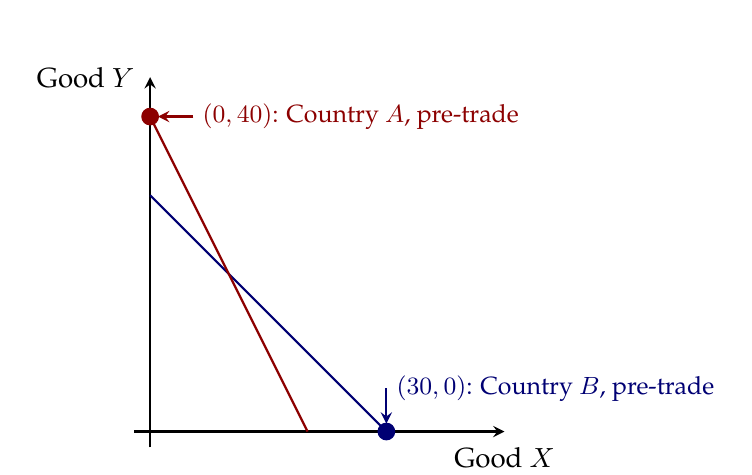
\begin{tikzpicture}[scale=1]
    % basics
    \draw [-stealth,color=black,thick] (-0.2,0) -- (4.5,0) node[below=2pt] {Good $X$};
    \draw [-stealth,color=black,thick] (0,-0.2) -- (0,4.5) node[left=2pt] {Good $Y$};
    
    % walrasian
    \draw[domain=0:3, blue!45!black, thick, variable=\x] plot ({\x}, {3-\x});
    % hicksian
    \draw[domain=0:2, red!55!black, thick, variable=\x] plot ({\x}, {4-2*\x});
    % intersection: \bar{p}
    \filldraw[red!55!black] (0,4) circle (3pt); 
    \filldraw[blue!45!black] (3,0) circle (3pt);
    
    % text
    \draw[-stealth,thick,red!55!black] (0.55,4) -- node[right=6pt] {\small $(0,40)$: Country $A$, pre-trade} (0.1,4);
    \draw[stealth-,thick,blue!45!black] (3,0.1) --  (3,0.55) node[right] {\small $(30,0)$: Country $B$, pre-trade}; % walrasian
\end{tikzpicture}
\end{center}

You might have already noticed that this PPF graph is exactly the specification used in Question 8 of Problem set 2, where the no-trade PPFs are:

\begin{table}[h!]
    \centering
    \begin{tabular}{ccc}
       & \textbf{\color{red!55!black}Country A} & \textbf{\color{blue!45!black}Country B} \\
     PPF & {\color{red!55!black} $Y = -2x+40$} & {\color{blue!45!black} $Y= -x+30$}
    \end{tabular}
\end{table}

Now we understand how the PPF is derived, we can just start from there from now on!

The 2 most important things of a PPF function is
\begin{itemize}
    \item[-] \textbf{slope}: 
    \begin{itemize}
        \item The country with the \underline{\textbf{flattest}} line has the comparative advantage in producing the good on \underline{\textbf{x-axis}}. In this example, \textbf{\color{blue!45!black}Country B}.
        \item The country with the \underline{\textbf{steepest}} line has the comparative advantage in producing the good on \underline{\textbf{y-axis}}. In this example, \textbf{\color{red!55!black}Country A}.
    \end{itemize}
    
    
    \item[-] \textbf{intersection with x- and y-axis}: assume full specialization, countries will only produce the good that they have a comparative advantage in producing (\textbf{\color{blue!45!black}Good X} for \textbf{\color{blue!45!black}Country B}, \textbf{\color{red!55!black}Good Y} for \textbf{\color{red!55!black}Country A}), hence we have
    \begin{itemize}
        \item The pre-trade bundle for \textbf{\color{blue!45!black}Country B} is ${(\color{blue!45!black}30,0)}$, the intersection of \textbf{\color{blue!45!black}Country B}'s line with \textbf{x-axis}, which represents \textbf{\color{blue!45!black}Good X}
        \item The pre-trade bundle for \textbf{\color{red!55!black}Country A} is ${(\color{red!55!black}0,40)}$, the intersection of \textbf{\color{red!55!black}Country A}'s line with \textbf{y-axis}, which represents \textbf{\color{red!55!black}Good Y}
    \end{itemize}
\end{itemize}

Now we can test whether a bundle can be achieved by trade or not. In Question 8, the potential post-trade bundle for Country A is $(10,22)$, let plot it

\begin{center}
    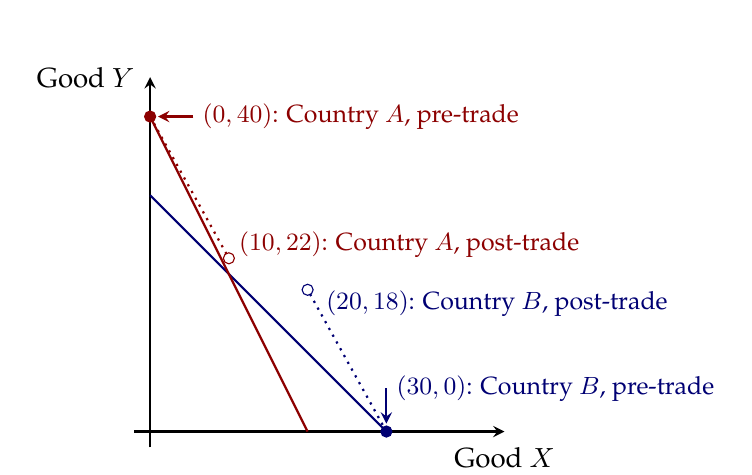
\begin{tikzpicture}[scale=1]
    % basics
    \draw [-stealth,color=black,thick] (-0.2,0) -- (4.5,0) node[below=2pt] {Good $X$};
    \draw [-stealth,color=black,thick] (0,-0.2) -- (0,4.5) node[left=2pt] {Good $Y$};
    
    % walrasian
    \draw[domain=0:3, blue!45!black, thick, variable=\x] plot ({\x}, {3-\x});
    % hicksian
    \draw[domain=0:2, red!55!black, thick, variable=\x] plot ({\x}, {4-2*\x});
    % intersection: \bar{p}
    \filldraw[red!55!black] (0,4) circle (2pt); 
    \filldraw[blue!45!black] (3,0) circle (2pt);
    \draw[red!55!black] (1,2.2) circle (2pt); 
    \draw[blue!45!black] (2,1.8) circle (2pt);
    
    \draw[thick, dotted, red!55!black] (0,4)-- (1,2.2) node[right,yshift=5pt] {\small $(10,22)$: Country $A$, post-trade};
    \draw[thick, dotted, blue!45!black] (3,0)--(2,1.8) node[right=3pt,yshift=-5pt] {\small $(20,18)$: Country $B$, post-trade};
    
    % text
    \draw[-stealth,thick,red!55!black] (0.55,4) -- node[right=6pt] {\small $(0,40)$: Country $A$, pre-trade} (0.1,4);
    \draw[stealth-,thick,blue!45!black] (3,0.1) --  (3,0.55) node[right] {\small $(30,0)$: Country $B$, pre-trade}; % walrasian
\end{tikzpicture}
\end{center}

Can this trade happen? Check 3 conditions:
\begin{itemize}
    \item[C1] \textbf{\textit{Is the new bundle achievable?}}
    
    We have 30 Good X, 40 Good Y, the new bundle for A is $(10,22)$, $10<30,22<40$, so it is achievable! 
    
    You can also calculate B's post trade bundle: $30-10 = 20>0$, $40-22=18 >0$, same logic.
    
    \item[C2] \textbf{\textit{Are both party happy?}}\footnote{Here, the more they produce, the happier they are. Later, we will reconsider "happy" with utility.}
    
    This is easy, just check whether the \textbf{new bundles} are \textbf{above} the pre-trade PPF lines respectively. Here, they both are!
    
    \item[C3] \textbf{\textit{Is the price reasonable?}}
    This is also easy, we verify it in 2 steps:
    \begin{itemize}
        \item[-] Step 1: calculate the price of trade, i.e., the slope of the dotted line in the graph 
        $$
        \frac{\lvert 22-40 \rvert}{\lvert 10- 0 \rvert} = \frac{18}{10} = 1.8
        $$
        \item[-] Step 2: check whether it is in between the slopes of the 2 pre-trade PPFs: $1.8<2, 1.8>1$, hence it is.
    \end{itemize}
    So the price is reasonable!
\end{itemize}

After checking the 3 conditions, we know this new bundle can be achieved by trade!

\underline{\textbf{\textit{Special remarks:}}}
The most confusing part of this procedure is probably the calculation of price. Just remember: \textbf{\underline{the opportunity cost is the slope, also the price}}. 

Let's look at the opportunity cost table again:
    \begin{table}[h!]
    \centering
        \begin{tabular}{c|cc}
             & Good X & Good Y \\
            \hline
            Country A & 2 & 0.5 \\
            Country B & 1 & 1
        \end{tabular}
    \end{table}
    
    To produce 1 unit of Good X, 
    \begin{itemize}
        \item Country A needs to give up 2 units of Good Y
        \item Country B needs to give up 1 units of Good Y
    \end{itemize}
    
    The price we calculated means that:
    $$
    \frac{\lvert 22-40 \rvert}{\lvert 10- 0 \rvert} = \frac{18}{10} = \frac{18  \text{ units of Y given up}}{\text{in exchange of } 10 \text{ units of X}} = 1.8
    $$
    this price has to be in between 1 and 2 here, because:
    \begin{itemize}
        \item if > 2: Country can just give 2 units of Y and produce 1 unit of X, instead of giving up more in trade to get 1 unit of X. 
        \item if < 1: Country can just give 1 unit of Y and produce 1 unit of X, instead of giving up 1 unit of Y but get less than 1 of unit of X in trade.
    \end{itemize}


\vspace{20pt}

Mathematically, it's easy: just calculate and compare the slopes. But the intuition behind these calculations is more important :)

%\newpage
%\bibliographystyle{plainnat}
%\bibliography{ref.bib}

\end{document}